\chapter{Architectural Details of ``Sapphire Rapids'' Processors}
The Sapphire Rapids family of server processors is the successor to the ``Ice Lake'' architecture.
Building up on the design of the Skylake~\cite{Schoene_2019_SKL} and Cascade Lake~\cite{Velten_2022_Rome_CLX} architectures, it is the first in Intels lineup of server processor to introduce a modular design containing four tiles in a 2x2 grid interconnected with EMIB structures.
The two variants of this processor are the 4th Generation Intel Xeon Scalable Processor and Xeon CPU Max Series with four additional HBM blocks~\cite{Intel_2021_Hotchips}.
Each tile contains up to 15 Golden Cove cores with a shared L3 cache connected by a mesh, an accelerator complex, two DDR5 memory busses, 20 PCIe Gen 5/CXL lanes and one UPI 2.0 link.
This structure enables the package to be used in a single memory domain or split into two or four sub-NUMA clusters~\cite{Intel_4th_gen_scalable}.
The accelerator complex can contain contains up to four different accelerators:
Data Streaming Accelerator (DSA) allows for memory move, fill and compare offloading.
QuickAssist Technology (QAT), allows for acceleration of cryptographic operations.
Dynamic Load Balancer (DLB), brings hardware acceleratored queues.
In-Memory Analytics Accelerator (IAA), allows for memory compression, encryption and filtering.~\cite{Yifan_2024_intel_accelerator_ecosystem,Yuan_2023_ISCA_tutorial,Intel_4th_gen_scalable}
Which accelerators are activated depend on the specific SKU, while Intel allows for the option to install licenses through an PCI express interface\footnote{\url{https://github.com/intel/intel-sdsi}}~\cite{Krenn_2025_Intel_on_demand}.
\figref{spr-overview} show a high level view of the processor.

\todoms{Add information about the cache sizes from the optimization reference manual.
Add information about new supported CPU instructions.}

\begin{figure}[]
    \centering
    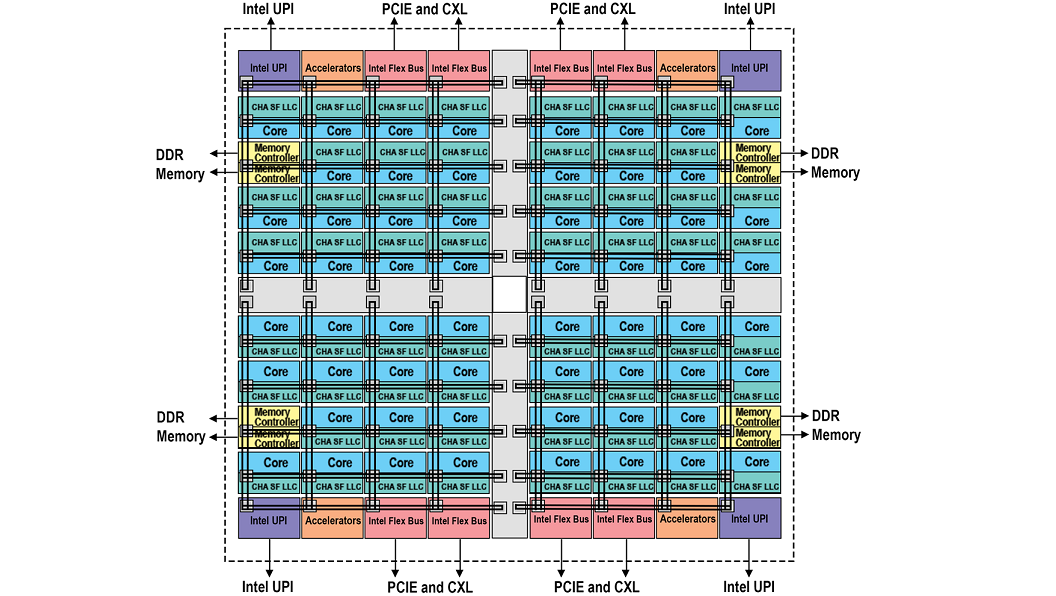
\includegraphics[width=\columnwidth]{fig/spr-uma.png}
    \caption{\label{fig:spr-overview}Block diagram of the 4th Generation Intel Xeon Scalable Processor from~\cite{Intel_4th_gen_scalable}.
Two mirrored tiles are arranged in a 2x2 grid, which are interconnected with EMIB structures to continue the mesh across the die boundaries.~\cite{Intel_2022_ISSCC}}
\end{figure}

\begin{figure}[]
    \begin{subfigure}[t]{0.45\linewidth}
        \centering
        \includegraphics[width=\linewidth]{fig/core-layout/socket0_tikz.pdf}
        \caption{Map of the first socket.}
    \end{subfigure}
    \hfill
    \begin{subfigure}[t]{0.45\linewidth}
        \centering
        \includegraphics[width=\linewidth]{fig/core-layout/socket1_tikz.pdf}
        \caption{Map of the second socket.}
    \end{subfigure}
    \caption{\label{fig:physical-layout}Physical layout of the processor with the IDs of the cache boxes and cores.
	Each box contains two numbers to represent the cache box id followed by a slash and the CPU id.
	Deactivated cache boxes and cores are marked with an X.}
\end{figure}

\section{Test System Details}
I performed all measurements on an Intel Xeon Platinum 8480+ dual socket server.
\tabref{test-system} shows details of the specific test system.
If not noted otherwise, all measurements on this processor are performed with hyperthreading and SNC-4 is activated.

\begin{table}[t]
	\centering
	\caption{\label{tab:test-system}Test system (hati) details}
	\begin{tabular}{rr}
		\toprule
		Processor	&	2x Intel Xeon Platinum 8480+ \\
		\rowcolor[HTML]{EFEFEF}Cores		&	2x 56 \\
		Available frequencies	&	\SI{800}{\MHz} -- \SI{3800}{\MHz} (\SI{2000}{\MHz} nominal) \\
		\rowcolor[HTML]{EFEFEF}L1-i and L1-d cache	&	112x (\SI{32}{\kibi\byte} + \SI{48}{\kibi\byte})\\
		L2 cache	&	112x \SI{2048}{\kibi\byte} \\
		\rowcolor[HTML]{EFEFEF}L3 cache	&	2x \SI{105}{\mebi\byte} (2d-mesh) \\
		Mainboard	&	Intel Corporation D50DNP1SB \\
		\rowcolor[HTML]{EFEFEF}Memory		&	16x Micron MTC20F2085S1RC48BA1  \\
		\rowcolor[HTML]{EFEFEF}&	\SI{4800}{\mega\hertz} \\
		Disk		&	Samsung MZQL27T6HBLA-00A07 \\
		\rowcolor[HTML]{EFEFEF}OS           &   Ubuntu 22.04 LTS \\
		Kernel          &   6.8.0-79-generic \\
		\bottomrule
		%\vspace{6mm}
	\end{tabular}
\end{table}

\todoms{Add citation for the papers that also do this, but somewhat differently.}
To find out which of the cores and caches are deactived I run the stream benchmark on each CPU, collect the Vertical Egress Events\footnote{\textbf{TxR\_VERT\_OCCUPANCY0} with AD - Agent 0 and AK - Agent 0: event=144,umask=0x03}, measuring the occupancy of the egress buffers in the mesh stop, and the Horizontal Egress Events\footnote{\textbf{TxR\_HORZ\_OCCUPANCY} with AD - Uncredited and AK: event=160,umask=0x03}, measuring the occupancy of the transgress buffers, for all cache boxes.
This measurement is performed using the default core frequency without the use of hyperthreading.
I use the vertical occupancy event to associate the cores to cache boxes.
The horizontal occupancy is used to find which cache boxes are in the same row.
I assume that at least one row contains all cores/caches and that the ids of the cache boxes are numbered sequentially.
This allows me to align the rows and columns to one another around a complete row.
As sub numa clustering is activated, the size of the rows and columns are bound to the size of a tile.
\figref{physical-layout} show the physical map of the processors core and cache slices positions on the test system.

\todoms{add test system details for ariel}

\section{Golden Cove Core Microarchitecture}

Unlike previous core microarchitectures~\cite{Intel_2020_Skylake_SP,Intel_2020_IceLake_SP} finding information about the interals of Golden Cove is quite difficult.
Major tech journalists~\cite{ServerTheHome_2023_SPR_Press,TechGage_2023_SPR_Press,HotHardware_2023_SPR_Press,Wccftech_2023_SPR_Press} have published slides presumably from the launch event in an coordinated press release at the 10th January 2023.
I was unable to find the original slide deck, requiring to take this information with extra caution.

Since I was unable to find public claims from Intel, I opted to measure individual components of the core, i.e. reorder buffer, load buffer, store buffer, register file sizes.
Henry Wong created a benchmark that can measure the reorder buffer size~\cite{Wong_2013_robsize} of the out-of-order engine, an essential component that falicitates reordering, idioms and move elimination.
The execution time of two independent pointer chasing loads is measured.
Different filler instructions are inserted between the two loads.
At some number of instructions the latency of the two loads increases since a limit of some structure in the out-of-order backend is hit.
I implemented the benchmark using C++ and the Asmjit~\cite{Kobalicek_AsmJit} library to generate assember kernels during runtime.~\footnote{\url{https://github.com/marenz2569/robsize}}
The loop is unrolled \SI{16}{} and repeated for \SI{2048}{} times.
I plot the minimum latency of \SI{16}{} executions of this benchmark with the number of filler instructions between \SI{16}{} and \SI{600}{}.
It is run on CPU 0 with hyperthreading disabled.
To verify the functionality against published values from a primary source~\cite{Intel_2020_Skylake_SP}, the measurement is repeated on a Skylake SP processor.

For measuring the reorder buffer \textbf{nop} instructions are inserted between the loads.
As~\figref{robsize-reorder} shows, the claim~\cite{ServerTheHome_2023_SPR_Press,Wccftech_2023_SPR_Press} of an out-of-order window with the size \SI{512}{} entries can clearly be validated.
To measure the size of the load and store buffers, I insert \textbf{mov} instructions taht load and store from memory to a register.
\figref{robsize-load} show a discrepancy between the claim~\cite{ServerTheHome_2023_SPR_Press,Wccftech_2023_SPR_Press} of 240 in-flight loads vs the 192 measured.
This has also been measured by Chips and Cheese~\cite{Chipsandcheese_2023_GoldenCove_Vector_Register}, they postulate that Intel is using a different mechanism for in-fligt loads.
Since different parts of the core are partitioned differently between threads, I assume that there could be partial static partitioning in the load queue.
This can however not be verified with the current version of the benchmark as it would require support for concurrent measurement on multiple threads of the same CPU.
\figref{robsize-store} shows that same result as the claim~\cite{ServerTheHome_2023_SPR_Press,Wccftech_2023_SPR_Press} of 112 stores.

\begin{figure}[]
    \centering
    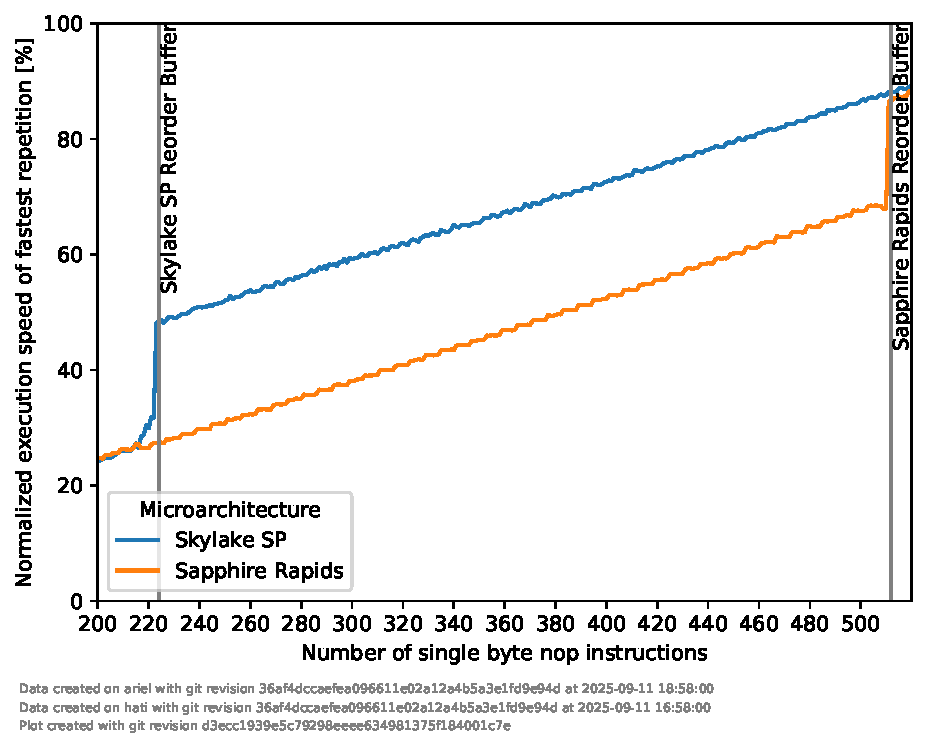
\includegraphics[width=0.8\columnwidth]{fig/robsize/reorder-buffer.pdf}
    \caption{\label{fig:robsize-reorder}Measurement of the reorder buffer size.}
\end{figure}
\begin{figure}[]
    \centering
    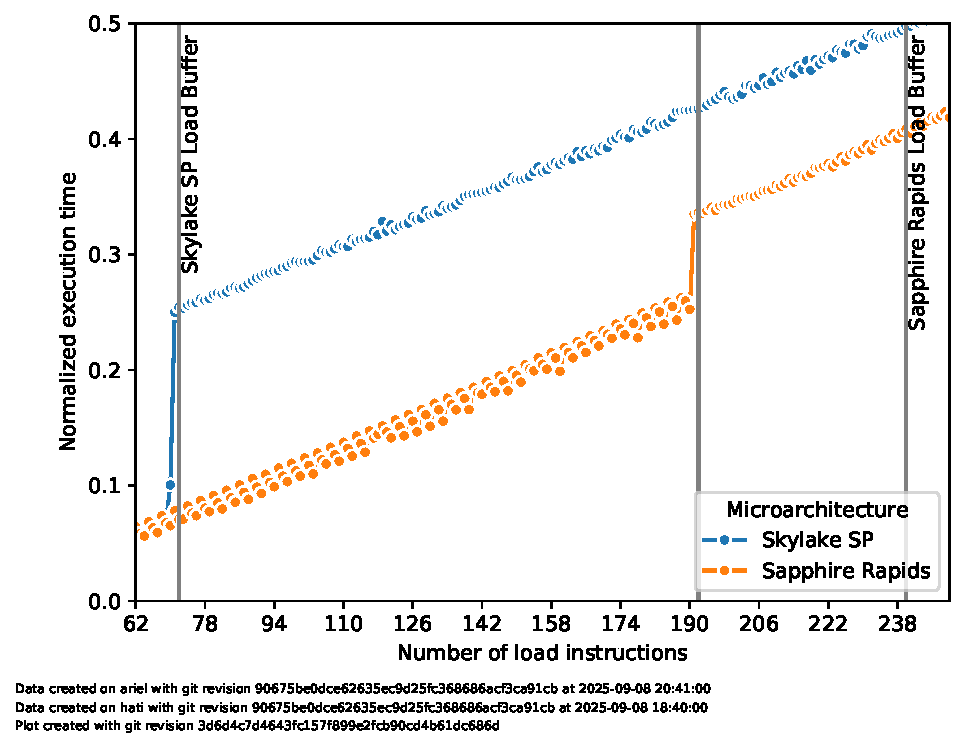
\includegraphics[width=0.8\columnwidth]{fig/robsize/load-buffer.pdf}
    \caption{\label{fig:robsize-load}Measurement of the load buffer size.}
\end{figure}
\begin{figure}[]
    \centering
    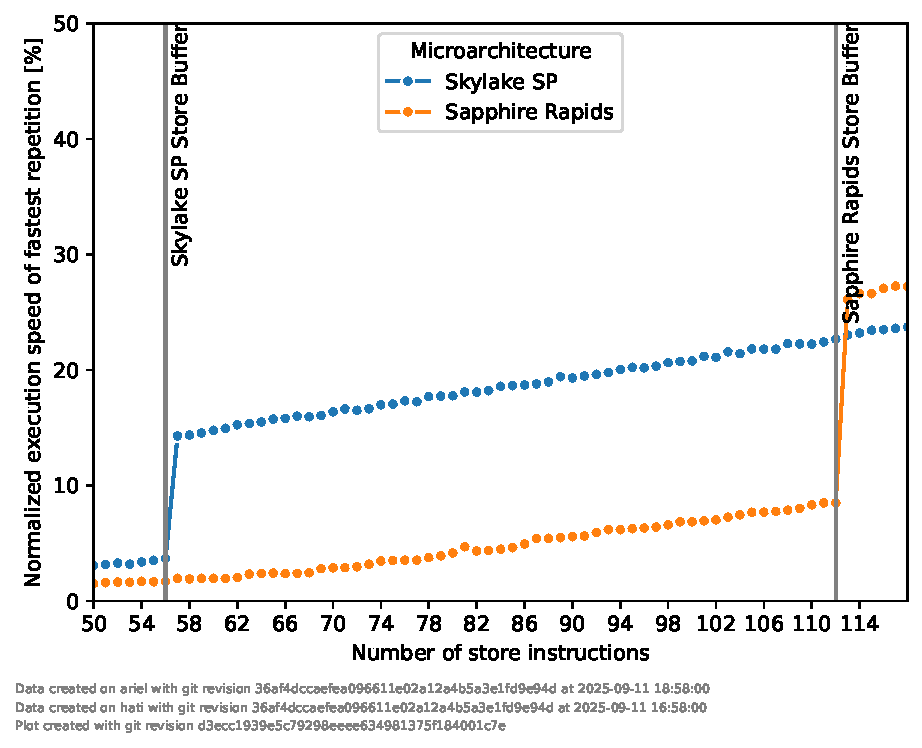
\includegraphics[width=0.8\columnwidth]{fig/robsize/store-buffer.pdf}
    \caption{\label{fig:robsize-store}Measurement of the store buffer size.}
\end{figure}

\begin{sidewaystable}[t]
	\centering
	\caption{\label{tab:micro-arch-params}Parameters of the Golden Cove Core Microarchitecture. Entries that are not from a primary source are either denoted with\\\checkmark if they have been verified, or ? if they need to be verfied.}
	\begin{tabular}{r|lll}
		\toprule
			&	Skylake & Golden Cove & Golden Cove Verified \\
		\rowcolor[HTML]{EFEFEF}Out-of-order Windows		& 224~\cite{Intel_2020_Skylake_SP} & 512~\cite{Intel_2021_Architecture_Day,ServerTheHome_2023_SPR_Press,Wccftech_2023_SPR_Press} & \checkmark~\figref{robsize-reorder} \\
		In-flight Loads & 72~\cite{Intel_2020_Skylake_SP} & 240~\cite{ServerTheHome_2023_SPR_Press,Wccftech_2023_SPR_Press} & 192 measured in~\figref{robsize-load} \\
		\rowcolor[HTML]{EFEFEF}In-flight Stores & 56~\cite{Intel_2020_Skylake_SP} & 112~\cite{ServerTheHome_2023_SPR_Press,Wccftech_2023_SPR_Press} & \checkmark~\figref{robsize-store} \\
		Register Files Integer & 180~\cite{Intel_2020_Skylake_SP} & 288~\cite{ServerTheHome_2023_SPR_Press,Wccftech_2023_SPR_Press} & ? \\
		\rowcolor[HTML]{EFEFEF}Register Files Floating Point & 168~\cite{Intel_2020_Skylake_SP} & 220 (512b), 320 (256b)~\cite{ServerTheHome_2023_SPR_Press,Wccftech_2023_SPR_Press} & ? \\
		Allocation Queue & 64/thread~\cite{Intel_2020_Skylake_SP} & 72/thread, 144 without SMT~\cite{Intel_2021_Architecture_Day,ServerTheHome_2023_SPR_Press,Wccftech_2023_SPR_Press} & \\
		μop Cache & & 4K~\cite{Intel_2021_Architecture_Day} & \\
		Decoder & & 32B decode size, 6 decoder, 8μop/cycle~\cite{Intel_2021_Architecture_Day} \\
		\rowcolor[HTML]{EFEFEF}L1i Cache & & & \\
		L1d Cache & & \\
		\rowcolor[HTML]{EFEFEF}L1d BW Load & 128~\cite{Intel_2020_Skylake_SP} & 3x256b or 2x512b~\cite{Intel_2021_Architecture_Day} & \\
		L1d BW Store & 64~\cite{Intel_2020_Skylake_SP} & & \\
		\rowcolor[HTML]{EFEFEF}L2 Unified TLB & 4K+2M: 1536 & 2K~\cite{ServerTheHome_2023_SPR_Press,Wccftech_2023_SPR_Press} & ? \\
		\rowcolor[HTML]{EFEFEF}  & 1G: 16~\cite{Intel_2020_Skylake_SP} & & \\
		Mid-level Cache & & & \\
		\bottomrule
		%\vspace{6mm}
	\end{tabular}
\end{sidewaystable}


\begin{figure}[]
    \centering
    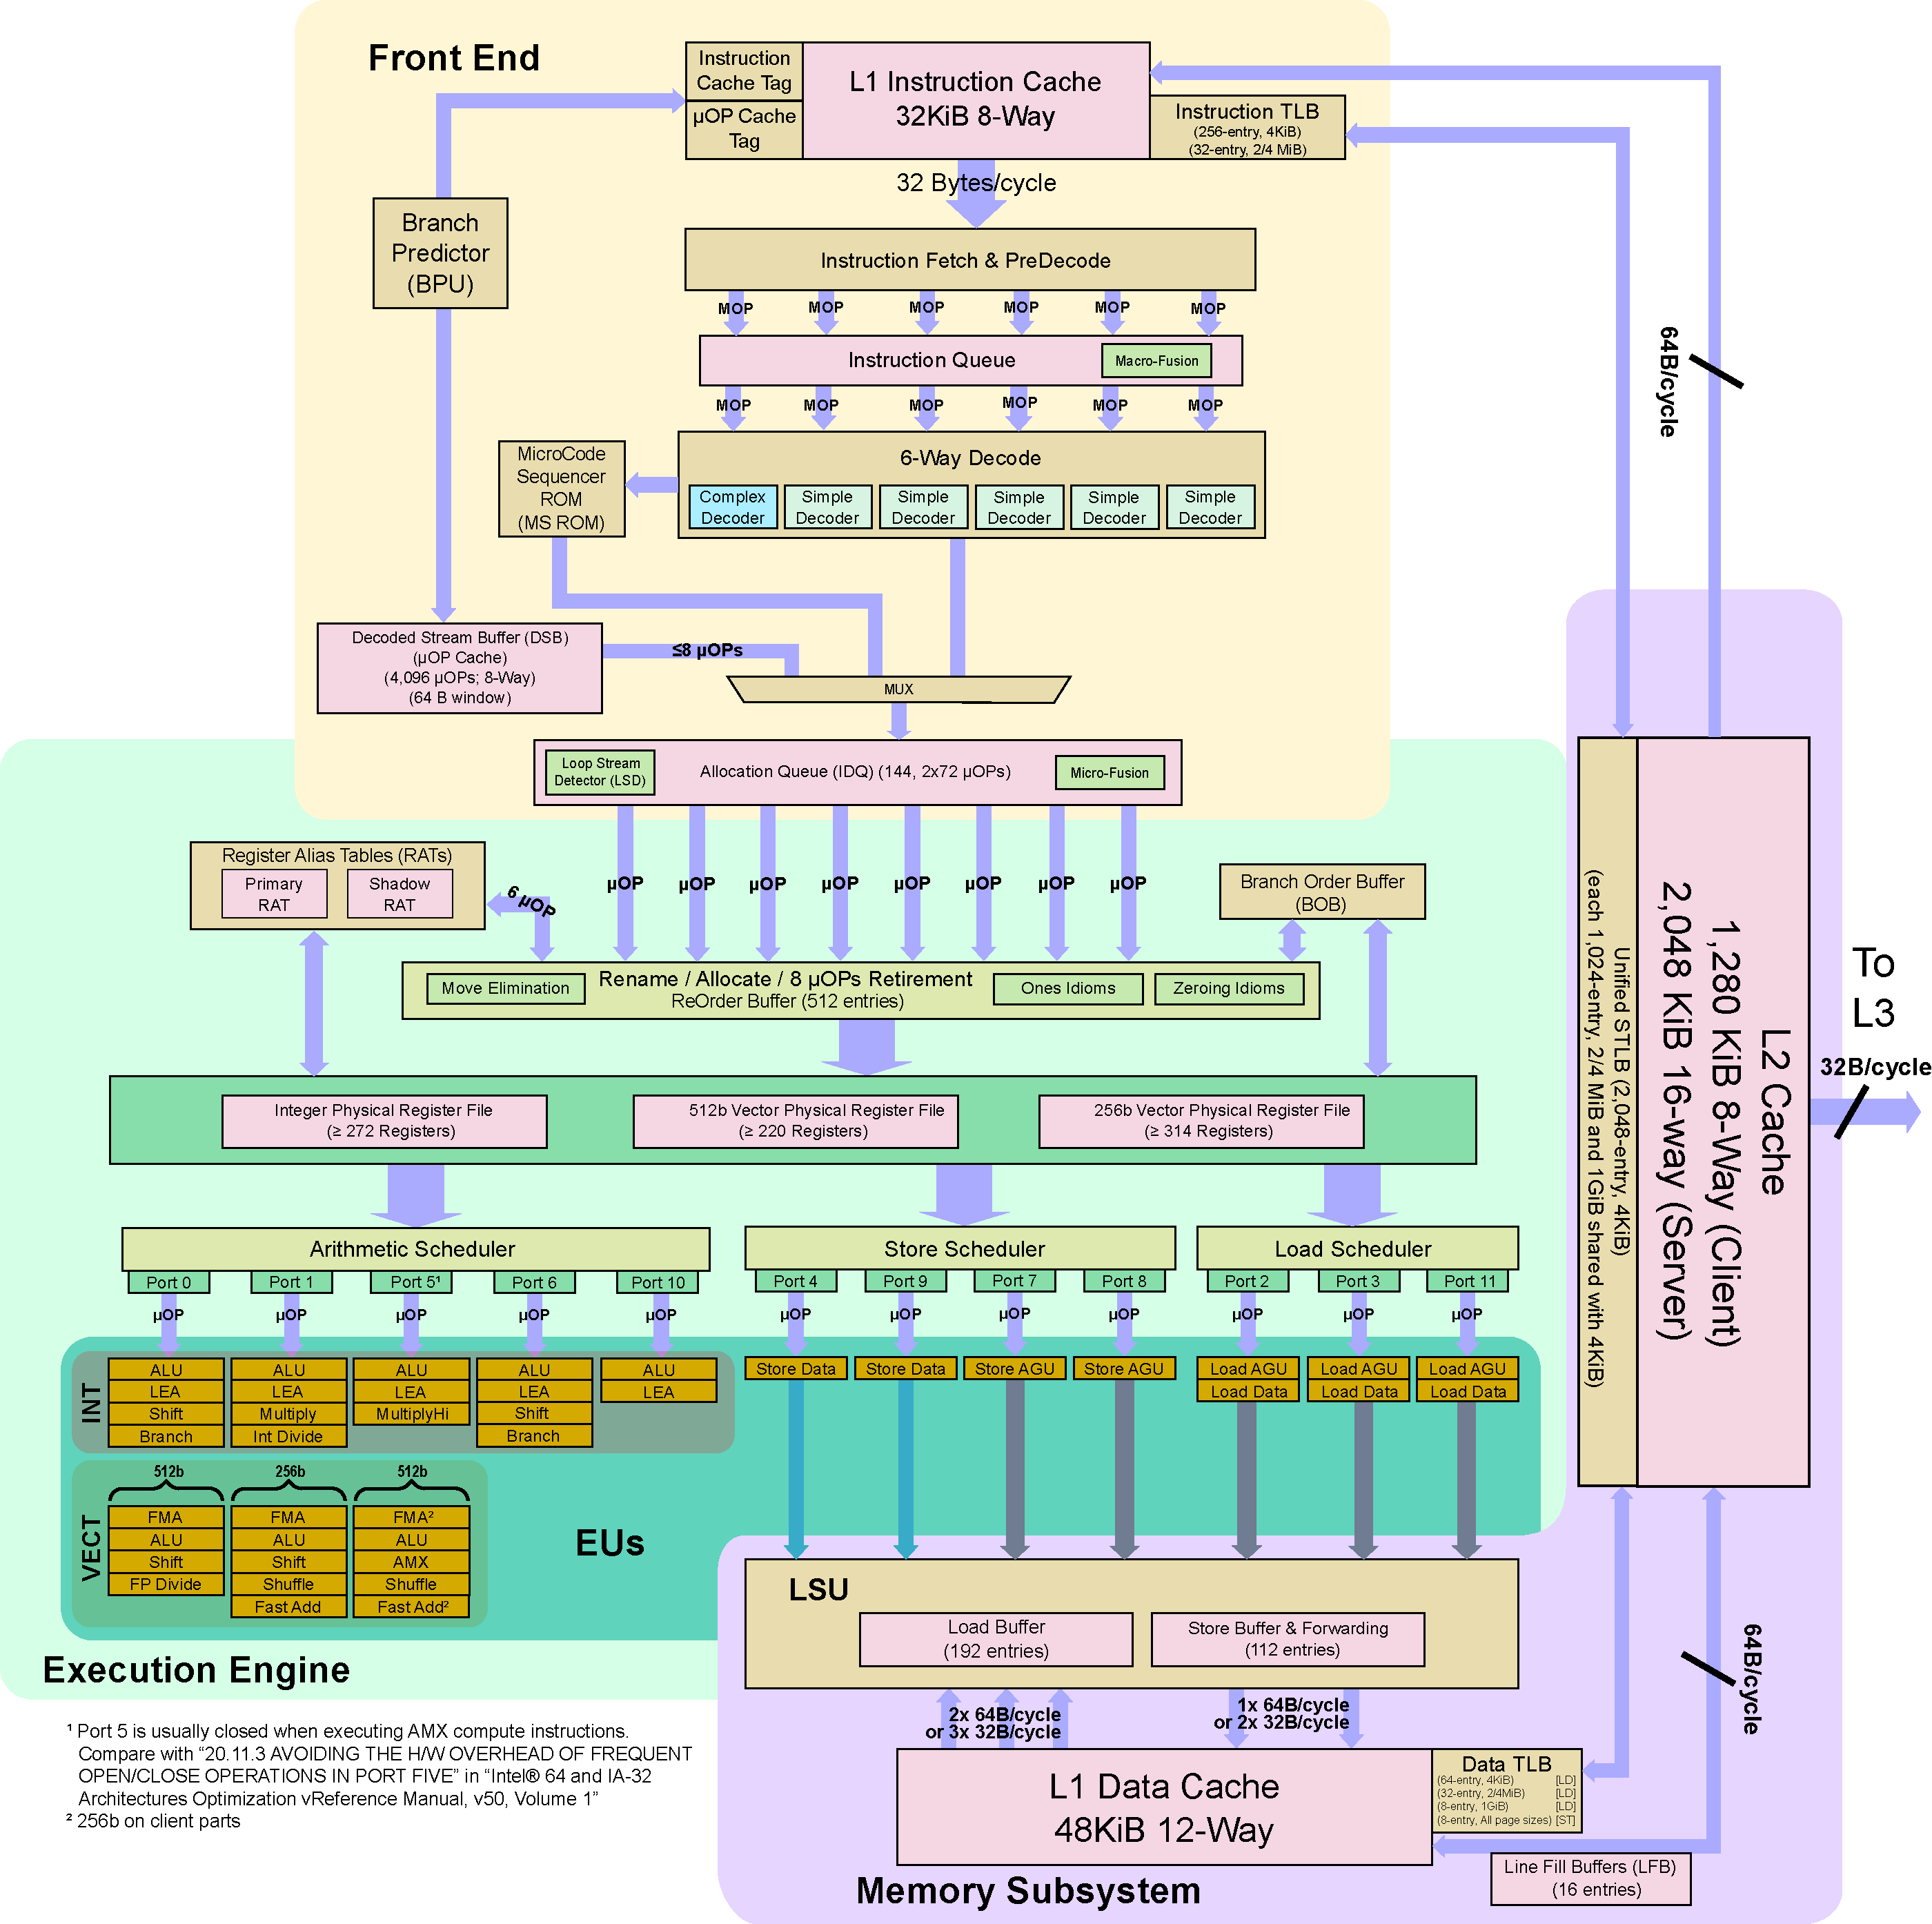
\includegraphics[width=\columnwidth]{fig/GoldenCoveCore.pdf}
    \caption{Block diagram of the Golden Cove Core.}
    \todoms{Measurements for the schedulers. How did the frontend change? Details of port 5 closing.}
\end{figure}